\documentclass[conference]{IEEEtran}
\IEEEoverridecommandlockouts

\usepackage[utf8]{inputenc}
\usepackage[T1]{fontenc}
\usepackage[spanish,es-tabla]{babel}
\usepackage{amsmath,amssymb}
\usepackage{graphicx}
\usepackage{booktabs}
\usepackage{array}
\usepackage{multirow}
\usepackage{url}
\usepackage{cite}
\usepackage{balance}
\usepackage{xcolor}

\newcommand{\aucroc}{AUC--ROC}
\newcommand{\aucpr}{AUC--PR}
\newcommand{\cpclass}{CP}
\newcommand{\fpclass}{FP}
\newcommand{\globalview}{\textit{global view}}
\newcommand{\localview}{\textit{local view}}
\newcommand{\etal}{\textit{et al.}}

\begin{document}

\title{Modelos Selectivos de Espacio de Estados para el \textit{Vetting} Automático de Candidatos a Exoplaneta en Curvas de Luz TESS}

\author{\IEEEauthorblockN{José F. Zumbado Ruiz, Jeremmy Aguilar Villanueva}
\IEEEauthorblockA{Escuela de Ingeniería en Computación\\
Instituto Tecnológico de Costa Rica\\
Cartago, Costa Rica\\
IC8104 Inteligencia Artificial, Semestre I 2026}}

\maketitle

\begin{abstract}
La misión TESS produce series temporales fotométricas de alta cadencia que requieren procesos de \textit{vetting} para separar candidatos planetarios reales de falsos positivos astrofísicos e instrumentales. Este trabajo evalúa si una arquitectura Mamba, basada en modelos selectivos de espacio de estados, ofrece una ventaja medible frente a baselines clásicos y convolucionales en la clasificación binaria de TESS Objects of Interest (TOIs). Se construyó un conjunto experimental de 1,576 objetos etiquetados como planeta confirmado (CP) o falso positivo (FP), dividido de forma estratificada por TIC ID en entrenamiento, validación y prueba sellada. Se compararon seis modelos: un baseline aleatorio estratificado, regresión logística con metadatos del catálogo, una CNN 1D inspirada en AstroNet, Mamba single-view, ExoMamba V1 con fusión tardía global-local, y una reproducción multirrama de AstroNet. En el conjunto de prueba sellado, el ensamble de cinco semillas de Mamba obtuvo \aucroc{} de 0.806, \aucpr{} de 0.711, F1 de 0.679 y \textit{recall} de 0.824, superando a la CNN single-branch en aproximadamente 20 puntos porcentuales de \aucroc{}. Además, el análisis de atribución mediante saliency, Integrated Gradients y oclusión mostró que el modelo concentra su decisión en los descensos fotométricos asociados a tránsitos. Los resultados sugieren que los modelos selectivos de estado son adecuados para vetting de secuencias largas bajo restricciones realistas de datos y hardware.
\end{abstract}

\begin{IEEEkeywords}
Exoplanetas, TESS, curvas de luz, Mamba, modelos de espacio de estados, aprendizaje profundo, vetting, inteligencia artificial explicable.
\end{IEEEkeywords}

\section{Introducción}

La detección y validación de exoplanetas por tránsito se basa en identificar reducciones pequeñas, periódicas y morfológicamente coherentes en el brillo observado de una estrella. La misión TESS (\textit{Transiting Exoplanet Survey Satellite}) fue diseñada para monitorear estrellas brillantes y generar curvas de luz con alta cadencia, lo que incrementa la disponibilidad de candidatos, pero también el volumen de señales que deben ser revisadas \cite{ricker2015tess}. En este contexto, la tarea de \textit{vetting} no consiste en detectar eventos desde cero, sino en decidir si un candidato ya propuesto por los catálogos de TOIs corresponde a un planeta confirmado o a un falso positivo.

El problema es especialmente desafiante porque las señales planetarias pueden confundirse con binarias eclipsantes, variabilidad estelar, ruido instrumental, errores de extracción fotométrica o artefactos asociados al procesamiento. Además, cada curva de luz global contiene aproximadamente 18,000 mediciones por sector, por lo que el modelo debe capturar simultáneamente patrones locales de tránsito y dependencias de largo alcance relacionadas con periodicidad, estabilidad y repetición de los eventos.

Los enfoques clásicos basados en variables resumidas del catálogo son interpretables y computacionalmente baratos, pero pueden perder información morfológica de la curva completa. Las redes convolucionales 1D, como las inspiradas en AstroNet \cite{shallue2018astronet}, capturan patrones locales, aunque su campo receptivo efectivo puede limitar la integración temporal de múltiples tránsitos separados por varios días. Por otro lado, los Transformers modelan dependencias globales mediante atención, pero su complejidad cuadrática respecto a la longitud de secuencia dificulta su uso directo en curvas largas \cite{vaswani2017attention}. Mamba surge como una alternativa eficiente al modelar secuencias mediante estados recurrentes selectivos con escalamiento lineal \cite{gu2023mamba}.

Este trabajo evalúa empíricamente la siguiente pregunta: ¿puede Mamba superar a baselines clásicos y convolucionales en el vetting de TOIs de TESS usando la curva de luz global completa? La contribución principal es una comparación controlada de modelos sobre el mismo protocolo de evaluación, con prueba sellada, múltiples semillas, análisis de error, calibración e interpretabilidad. Las contribuciones específicas son:

\begin{itemize}
    \item Se organiza un conjunto de 1,576 TICs etiquetados como CP o FP, con división estratificada por estrella para prevenir fuga de información entre sectores.
    \item Se implementa una escalera experimental de seis modelos que separa el aporte de metadatos, CNN, Mamba, vista local y fusión global-local.
    \item Se reportan resultados en prueba sellada, incluyendo \aucroc{}, \aucpr{}, F1, \textit{recall}, precisión, Brier score y matrices de confusión.
    \item Se aplica explicabilidad post-hoc con saliency, Integrated Gradients y oclusión para verificar si el modelo atiende regiones físicamente plausibles de la curva.
\end{itemize}

\section{Trabajos Relacionados}

El uso de aprendizaje profundo para vetting de exoplanetas ha sido impulsado por AstroNet, una arquitectura convolucional multirrama aplicada originalmente a curvas de luz de Kepler \cite{shallue2018astronet}. Su diseño combina una vista global de la señal y una vista local centrada en el tránsito plegado en fase. Esta combinación permite conservar el contexto orbital y, al mismo tiempo, analizar con mayor resolución la morfología del evento principal.

Trabajos posteriores, como ExoMiner, extendieron esta línea incorporando múltiples fuentes de información e interpretabilidad para clasificar candidatos planetarios con alta precisión \cite{valizadegan2022exominer}. Estos métodos muestran que la combinación de fotometría, variables estelares y rasgos derivados puede mejorar el desempeño del vetting automático. Sin embargo, muchos sistemas de referencia se benefician de conjuntos de datos más grandes, entrenamiento previo sobre Kepler o arquitecturas con múltiples ramas especializadas.

En el área general de modelado secuencial, los Transformers reemplazaron la recurrencia tradicional por mecanismos de autoatención, logrando avances significativos en tareas de lenguaje y secuencia \cite{vaswani2017attention}. No obstante, la autoatención estándar escala como $O(L^2)$ para una secuencia de longitud $L$, lo cual puede ser costoso para curvas de luz extensas. Mamba propone una familia de modelos selectivos de espacio de estados que mantiene complejidad lineal y permite propagar o descartar información en función del contenido de la entrada \cite{gu2023mamba}. Esta propiedad es relevante para TESS, donde gran parte de la curva puede contener ruido o regiones no informativas, mientras que pocos segmentos contienen evidencia de tránsito.

Finalmente, la explicabilidad se vuelve relevante porque el objetivo científico no es solo maximizar una métrica, sino justificar si el modelo está aprendiendo señales astronómicas. Integrated Gradients formaliza un método de atribución axiomático para redes profundas \cite{sundararajan2017ig}, mientras que la sensibilidad por oclusión evalúa el cambio de la salida cuando se enmascaran regiones de la entrada. En este trabajo se combinan ambos enfoques con saliency clásico para inspeccionar decisiones de Mamba sobre ejemplos CP y FP.

\section{Fundamento Teórico}

\subsection{Curvas de luz y vetting de TOIs}

Una curva de luz es una serie temporal $x = (x_1, x_2, \ldots, x_L)$ que representa el flujo estelar medido a lo largo del tiempo. En el caso de un tránsito, la señal esperada es una depresión temporal, aproximadamente periódica, causada por el paso de un planeta frente a su estrella. La Fig.~\ref{fig:transit_concept} resume este principio.

\begin{figure}[htbp]
    \centering
    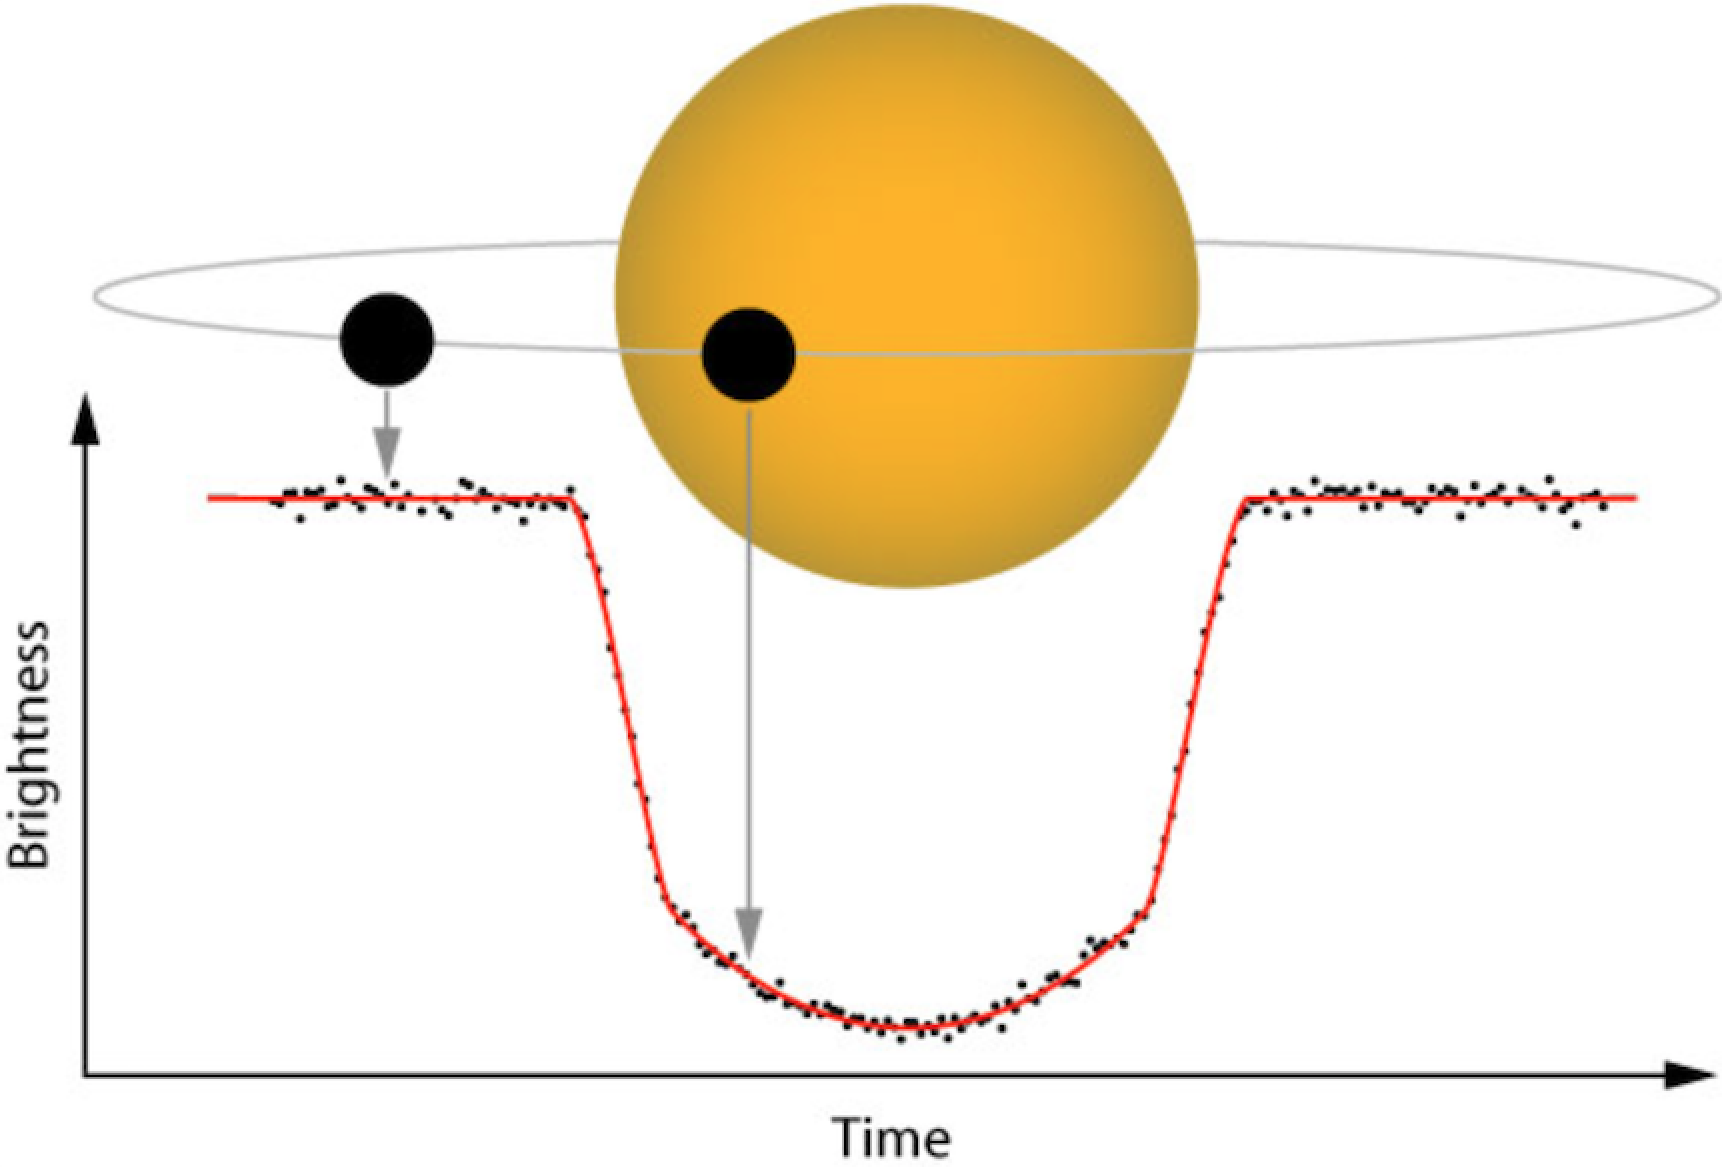
\includegraphics[width=0.95\linewidth]{figures/concept_lightcurve_transit.png}
    \caption{Representación conceptual de una señal de tránsito en una curva de luz. El vetting automático busca distinguir caídas compatibles con planetas de falsos positivos y artefactos.}
    \label{fig:transit_concept}
\end{figure}

En este estudio se utiliza el identificador TIC (\textit{TESS Input Catalog}) como unidad de separación entre conjuntos. Esto es importante porque una misma estrella puede aparecer en varios sectores; separar por observación, en lugar de por TIC, permitiría que información de la misma estrella aparezca simultáneamente en entrenamiento y prueba.

\subsection{Métricas de evaluación}

La tarea se formula como clasificación binaria, donde $y=1$ representa CP y $y=0$ representa FP. Debido al desbalance entre clases, la exactitud no se usa como métrica principal. Se priorizan métricas sensibles al ranking y a la clase positiva:

\begin{equation}
\text{Recall}=\frac{TP}{TP+FN},\qquad
\text{Precision}=\frac{TP}{TP+FP}.
\end{equation}

El puntaje F1 se define como

\begin{equation}
F_1=\frac{2\cdot \text{Precision}\cdot \text{Recall}}{\text{Precision}+\text{Recall}}.
\end{equation}

Además, se reporta \aucroc{}, que mide la capacidad del modelo para asignar mayor probabilidad a un CP que a un FP, y el Brier score, que cuantifica la calidad de calibración probabilística:

\begin{equation}
\text{Brier}=\frac{1}{N}\sum_{i=1}^{N}(\hat{p}_i-y_i)^2.
\end{equation}

\subsection{Mamba como modelo de estado selectivo}

Mamba modela una secuencia mediante una actualización recurrente de estado, pero con parámetros dependientes de la entrada. De forma simplificada, su dinámica puede expresarse como

\begin{equation}
 h_t = \bar{A}_t h_{t-1}+\bar{B}_t x_t, \qquad y_t=C_t h_t,
\end{equation}

donde $h_t$ es un estado latente y $\bar{A}_t$, $\bar{B}_t$ y $C_t$ son funciones del contenido observado. Esta selectividad permite filtrar regiones poco informativas y retener evidencia temporal relevante. A diferencia de una CNN, que aplica filtros locales, Mamba puede integrar información a lo largo de toda la secuencia con complejidad lineal en $L$ \cite{gu2023mamba}.

\section{Metodología}

\subsection{Conjunto de datos}

El conjunto experimental se construyó a partir de TOIs de TESS con etiquetas CP y FP. Tras el filtrado de calidad, se obtuvieron 1,576 TICs: 603 CP y 973 FP. Para los modelos que requieren vista local plegada en fase se definió un subconjunto Tier 2 de 1,406 objetos con periodo, época y duración válidos. La Tabla~\ref{tab:splits} resume la división por split.

\begin{table}[htbp]
\centering
\caption{Distribución de datos por split y subconjunto experimental.}
\label{tab:splits}
\resizebox{\linewidth}{!}{%
\begin{tabular}{lrrrr}
\toprule
\textbf{Split} & \textbf{Tier 1 N} & \textbf{CP/FP} & \textbf{Tier 2 N} & \textbf{CP/FP} \\
\midrule
Entrenamiento & 1103 & 422/681 & 985 & 376/609 \\
Validación & 236 & 90/146 & 211 & 77/134 \\
Prueba sellada & 237 & 91/146 & 210 & 78/132 \\
Total & 1576 & 603/973 & 1406 & 531/875 \\
\bottomrule
\end{tabular}}
\end{table}

La división se realizó en proporción 70/15/15 y se estratificó por clase. El conjunto de prueba se mantuvo sellado: cada modelo se evaluó una única vez sobre test, luego de cerrar hiperparámetros con validación.

\subsection{Representaciones de entrada}

La \globalview{} corresponde a la curva de luz PDCSAP normalizada por la mediana de cada curva y remuestreada a $L=18,000$ puntos. La normalización se realiza individualmente por TIC para evitar que estadísticas globales del conjunto contaminen los splits.

Para los modelos Tier 2 se construyó una \localview{} mediante plegado en fase. Dado un periodo orbital $P$, una época de tránsito $T_0$ y una duración $D$, se define

\begin{equation}
\phi(t)=\frac{(t-T_0)\bmod P}{P}.
\end{equation}

Luego se conserva una ventana centrada en el tránsito y se discretiza a 201 puntos. Esta vista busca aumentar la relación señal-ruido al alinear múltiples tránsitos sobre una misma fase.

\subsection{Modelos evaluados}

Se implementó una escalera experimental con seis modelos, diseñada para aislar el efecto de cada componente:

\begin{enumerate}
    \item \textbf{Random estratificado:} baseline sin entrenamiento que predice según el prior de clase.
    \item \textbf{Regresión logística de catálogo:} modelo lineal con periodo orbital, profundidad de tránsito y magnitud estelar.
    \item \textbf{CNN single-branch:} red convolucional 1D inspirada en AstroNet, aplicada únicamente a la vista global.
    \item \textbf{Mamba single-view:} modelo principal, con embedding lineal $1\rightarrow64$, cuatro bloques Mamba y pooling global.
    \item \textbf{ExoMamba V1:} fusión tardía de Mamba global con una CNN local ligera.
    \item \textbf{AstroNet multibranch:} reproducción adaptada de la arquitectura global-local con ramas convolucionales.
\end{enumerate}

La CNN single-branch usa cuatro bloques Conv1D--BatchNorm--ReLU--MaxPool y un clasificador denso. Mamba emplea $d_{model}=64$, cuatro capas, $d_{state}=16$, convolución interna de tamaño 4 y factor de expansión 2, para un total de 131,393 parámetros. AstroNet multibranch contiene aproximadamente 1.34 millones de parámetros, mientras que ExoMamba V1 contiene cerca de 153 mil.

\subsection{Entrenamiento y optimización}

El entrenamiento se realizó bajo restricciones de hardware equivalentes a una GPU RTX 3050 de 4 GB. Se usó búsqueda aleatoria ad hoc sobre Mamba, evaluando tasas de aprendizaje en $\{10^{-3},1.5\times10^{-3},2\times10^{-3},3\times10^{-3}\}$, paciencia de early stopping, tamaño de estado y uso de augmentation. La configuración seleccionada utilizó learning rate $1.5\times10^{-3}$, $d_{state}=16$ y gradient clipping con norma máxima de 1.0.

No se aplicó K-fold cross-validation porque el costo por configuración habría sido prohibitivo para el hardware disponible. Como alternativa, se entrenaron múltiples semillas independientes. Para Mamba se usaron cinco semillas y se construyó un ensamble por promedio de probabilidades. Para ExoMamba V1 y AstroNet se usaron tres semillas.

\section{Experimentos}

\subsection{Protocolo de evaluación}

Todos los modelos se evaluaron en el split de prueba sellado. Las métricas se calcularon con umbral 0.5 para F1, \textit{recall}, precisión y matriz de confusión. Para \aucroc{} y \aucpr{} se utilizaron las probabilidades continuas. El ensamble se obtuvo promediando las probabilidades predichas por las semillas disponibles antes de aplicar el umbral.

\subsection{Resultados principales}

La Tabla~\ref{tab:results} presenta los resultados principales. En Tier 1, Mamba supera claramente al baseline aleatorio, a la regresión logística de catálogo y a la CNN single-branch. El ensamble de cinco semillas alcanza \aucroc{} de 0.806, lo que representa una mejora absoluta de aproximadamente 0.202 respecto a la CNN single-branch.

\begin{table*}[htbp]
\centering
\caption{Resultados en prueba sellada. Tier 1 usa solo vista global ($N_{test}=237$); Tier 2 usa vista global y local en un subconjunto estricto ($N_{test}=210$).}
\label{tab:results}
\resizebox{\textwidth}{!}{%
\begin{tabular}{llrrrrrrr}
\toprule
\textbf{Tier} & \textbf{Modelo} & \textbf{\aucroc{}} & \textbf{\aucpr{}} & \textbf{F1} & \textbf{Recall} & \textbf{Precision} & \textbf{Brier} & \textbf{Parámetros} \\
\midrule
1 & Random estratificado & 0.500 & -- & 0.000 & 0.000 & -- & 0.237 & 0 \\
1 & Regresión logística catálogo & 0.605 & 0.464 & 0.486 & 0.571 & 0.423 & -- & $\sim$10 \\
1 & CNN single-branch & 0.604 & 0.551 & 0.539 & 0.758 & 0.418 & -- & 62,881 \\
1 & Mamba single locked & 0.763 & 0.650 & 0.633 & 0.835 & 0.510 & 0.210 & 131,393 \\
1 & Mamba multi-seed mean $\pm$ std & $0.750\pm0.065$ & -- & -- & -- & -- & -- & 131,393 \\
1 & \textbf{Mamba ensemble} & \textbf{0.806} & \textbf{0.711} & \textbf{0.679} & \textbf{0.824} & \textbf{0.577} & \textbf{0.192} & $5\times$131,393 \\
1 & Mamba best seed 789 & 0.810 & 0.722 & 0.661 & 0.802 & 0.562 & 0.190 & 131,393 \\
\midrule
2 & ExoMamba V1 ensemble & 0.460 & 0.371 & 0.542 & 1.000 & 0.371 & 0.254 & $3\times$153K \\
2 & AstroNet multibranch ensemble & 0.716 & 0.582 & 0.563 & 0.603 & 0.528 & 0.217 & $3\times$1.34M \\
\bottomrule
\end{tabular}}
\end{table*}

La Fig.~\ref{fig:roc} muestra la comparación ROC de los modelos Tier 1. La curva de Mamba se mantiene por encima de las alternativas clásicas y convolucionales, lo que confirma que la mejora no depende de un único umbral de decisión.

\begin{figure}[htbp]
    \centering
    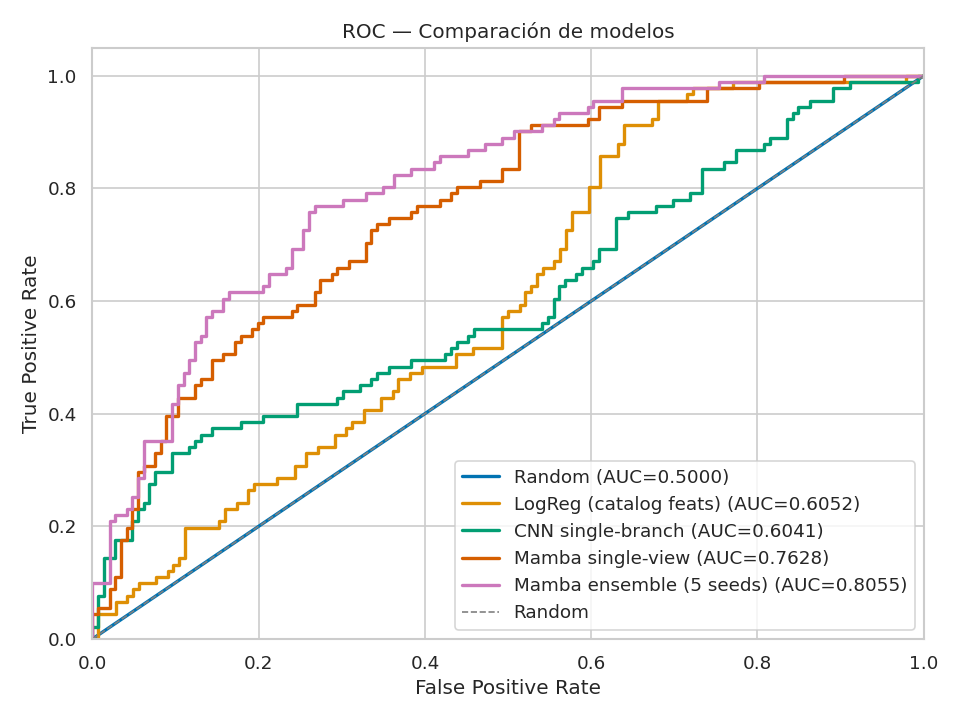
\includegraphics[width=0.98\linewidth]{figures/roc_tier1.png}
    \caption{Curvas ROC comparativas para los modelos Tier 1. El ensamble de Mamba alcanza la mayor área bajo la curva.}
    \label{fig:roc}
\end{figure}

\subsection{Matriz de confusión y calibración}

La Fig.~\ref{fig:confcal} presenta la matriz de confusión y la curva de calibración del ensamble Mamba. En comparación con la CNN single-branch, Mamba incrementa los verdaderos negativos de 50 a 91 y reduce los falsos positivos de 96 a 55. Esto indica que la mejora principal no es solo detectar más CP, sino descartar con mayor precisión falsos positivos.

\begin{figure*}[htbp]
\centering
\begin{minipage}{0.47\textwidth}
    \centering
    
\includegraphics[width=0.98\linewidth]{results/mamba_ensemble/confusion_matrix.png}
\end{minipage}
\hfill
\begin{minipage}{0.47\textwidth}
    \centering
    
\includegraphics[width=0.98\linewidth]{results/mamba_ensemble/calibration.png}
\end{minipage}
\caption{Matriz de confusión y calibración probabilística del ensamble Mamba en prueba sellada.}
\label{fig:confcal}
\end{figure*}

\begin{table}[htbp]
\centering
\caption{Comparación de conteos de error entre Mamba ensemble y CNN single-branch en el mismo test Tier 1.}
\label{tab:conf_compare}
\resizebox{\linewidth}{!}{%
\begin{tabular}{lrrr}
\toprule
\textbf{Cuadrante} & \textbf{Mamba} & \textbf{CNN} & \textbf{$\Delta$} \\
\midrule
TP & 75 & 69 & +6 \\
TN & 91 & 50 & +41 \\
FN & 16 & 22 & -6 \\
FP & 55 & 96 & -41 \\
\bottomrule
\end{tabular}}
\end{table}

\subsection{Análisis de errores}

La Fig.~\ref{fig:error_analysis} resume dos diagnósticos sobre el ensamble Mamba. La distribución de probabilidades muestra solapamiento entre clases principalmente en el intervalo $\hat{p}\in[0.4,0.6]$, donde se concentran las decisiones ambiguas. El análisis por variable física identifica mayor tasa de error para profundidades de tránsito entre 136 y 770 ppm, un régimen compatible con señales de baja relación señal-ruido.

\begin{figure*}[htbp]
\centering
\begin{minipage}{0.47\textwidth}
    \centering
    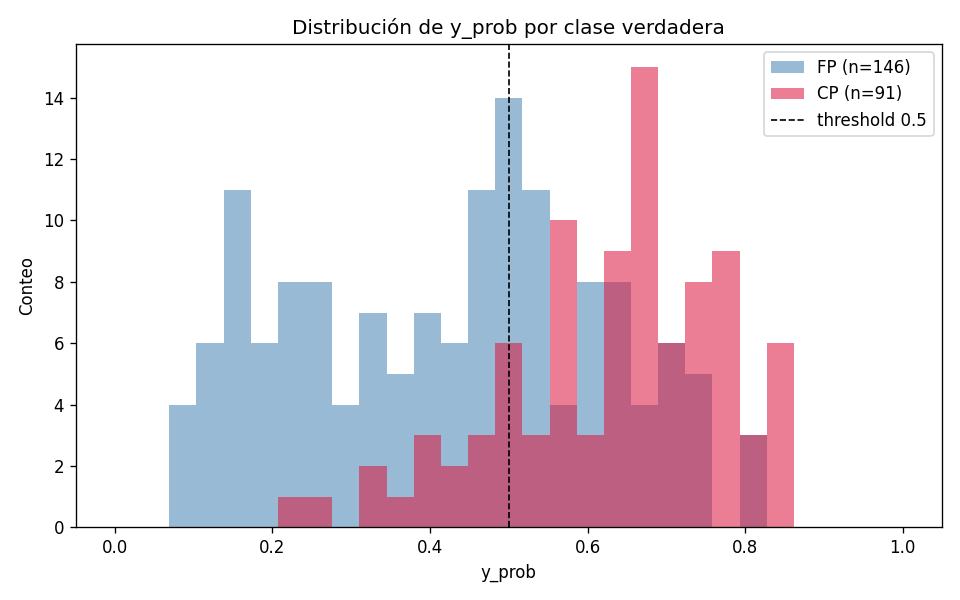
\includegraphics[width=0.98\linewidth]{results/error_analysis/mamba_ensemble/prob_histogram.png}
\end{minipage}
\hfill
\begin{minipage}{0.47\textwidth}
    \centering
    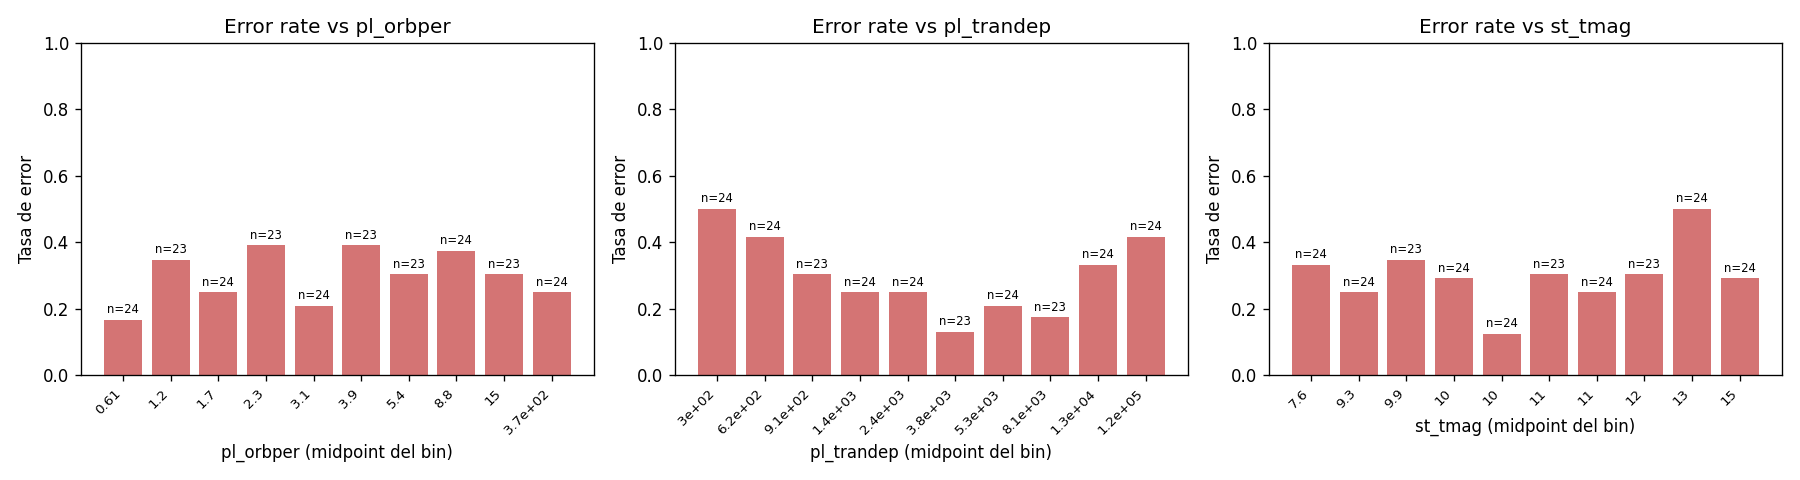
\includegraphics[width=0.98\linewidth]{results/error_analysis/mamba_ensemble/error_rate_by_feature.png}
\end{minipage}
\caption{Análisis de errores del ensamble Mamba: distribución de probabilidades por clase verdadera y tasa de error por bins de variables físicas.}
\label{fig:error_analysis}
\end{figure*}

\section{Interpretabilidad}

Se aplicaron tres métodos de atribución sobre el modelo Mamba con mejor semilla individual: saliency por gradiente, Integrated Gradients y sensibilidad por oclusión. Saliency calcula la magnitud de la derivada local del logit respecto a cada punto de la curva:

\begin{equation}
\text{Sal}(x_t)=\left|\frac{\partial f(x)}{\partial x_t}\right|.
\end{equation}

Integrated Gradients estima la contribución acumulada desde una línea base $x'$ hasta la entrada observada $x$:

\begin{equation}
\text{IG}(x_t)=(x_t-x'_t)\int_0^1 \frac{\partial f(x'+\alpha(x-x'))}{\partial x_t}d\alpha.
\end{equation}

La oclusión mide el cambio del logit al reemplazar ventanas de la curva por una línea base. Estos métodos son complementarios: los gradientes capturan sensibilidad local, Integrated Gradients reduce problemas de saturación, y la oclusión evalúa importancia por intervención.

La Fig.~\ref{fig:xai} muestra ocho casos de prueba, seleccionados como los dos ejemplos más confiados de cada cuadrante TP, TN, FN y FP. En los verdaderos positivos, las atribuciones se concentran en dips compatibles con tránsito, lo que sugiere que Mamba aprende señales físicamente plausibles. En falsos positivos, la atribución también se concentra en caídas pronunciadas; esto indica que el modelo detecta eventos reales en la curva, pero no siempre separa tránsitos planetarios de eclipses binarios cuando la morfología es similar.

\begin{figure*}[htbp]
    \centering
    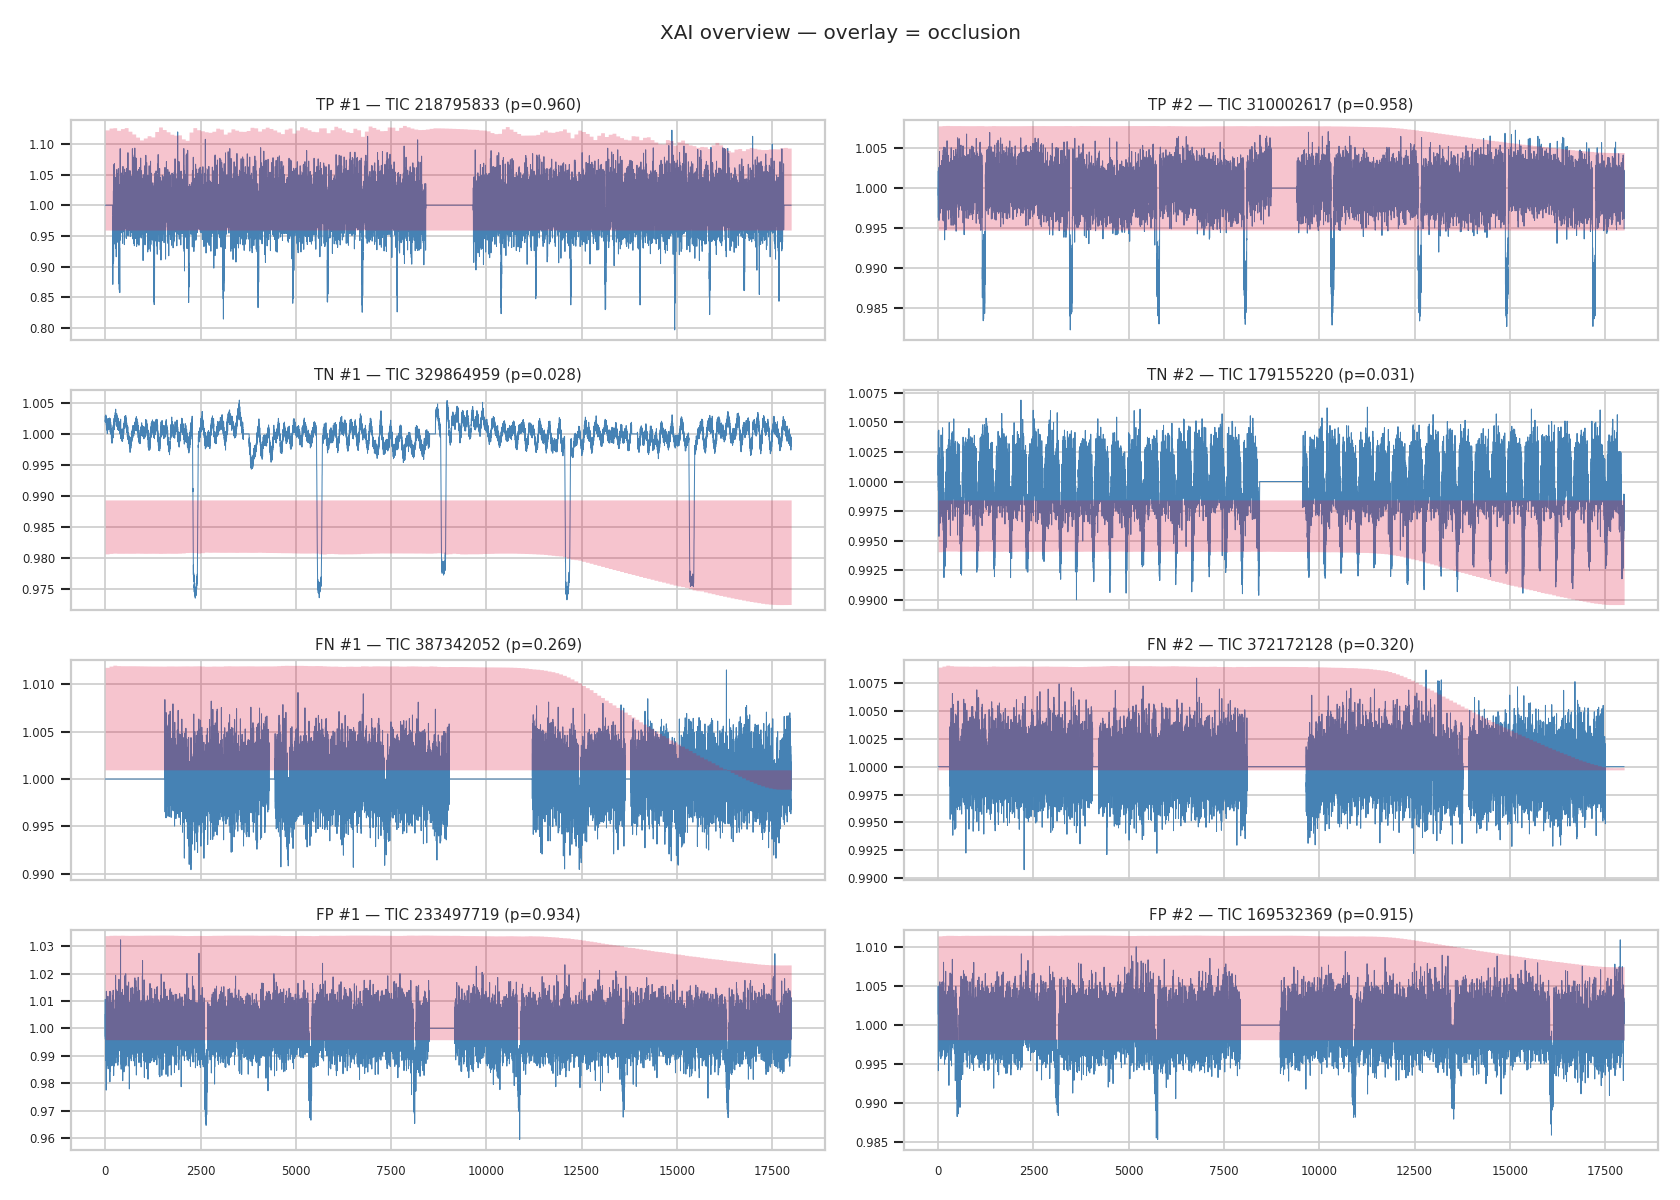
\includegraphics[width=0.98\textwidth]{figures/xai/mamba_seed789/_summary.png}
    \caption{Resumen de explicabilidad para ocho casos del test y tres métodos de atribución. La concentración de atribución en dips de tránsito para TP apoya la plausibilidad física de las decisiones del modelo.}
    \label{fig:xai}
\end{figure*}

\section{Discusión}

\subsection{Ventaja de Mamba en secuencias largas}

La diferencia entre Mamba y la CNN single-branch no se explica únicamente por el número de parámetros: Mamba tiene cerca del doble de parámetros que la CNN, pero supera su \aucroc{} por más de 20 puntos porcentuales. La explicación más plausible es arquitectural. Una CNN 1D aprende filtros locales y expande su campo receptivo por apilamiento y pooling, mientras que Mamba propaga un estado latente a lo largo de toda la curva. Para vetting de TESS, donde la evidencia puede estar distribuida en varios tránsitos separados por días, esta capacidad de integración temporal es fundamental.

\subsection{Papel de la vista local}

AstroNet multibranch supera al CNN single-branch, lo cual respalda que el plegado en fase aporta información útil. Sin embargo, AstroNet queda por debajo del ensamble Mamba. Esto sugiere que, en un dataset relativamente pequeño y sin transfer learning desde Kepler, una arquitectura convolucional más grande no necesariamente compensa la ausencia de modelado explícito de largo alcance sobre los 18,000 puntos de la vista global.

\subsection{Ablación negativa de ExoMamba V1}

ExoMamba V1, que fusiona Mamba global y CNN local mediante concatenación tardía, obtuvo \aucroc{} menor que 0.5 en el ensamble de tres semillas. Este resultado no debe interpretarse como evidencia contra la fusión global-local, sino contra una fusión ingenua. La arquitectura pasó pruebas de sobreajuste en subconjuntos pequeños, por lo que el problema probable se encuentra en la dinámica de entrenamiento y en el operador de fusión. Métodos como cross-attention, FiLM o gating learnable podrían permitir una interacción más estable entre ramas.

\subsection{Limitaciones}

El estudio tiene cinco limitaciones principales. Primero, el dataset final contiene 1,576 objetos, menor que los conjuntos usados por sistemas entrenados sobre Kepler. Segundo, no se utilizó transfer learning desde modelos preentrenados. Tercero, no se ejecutó K-fold cross-validation por costo computacional; se sustituyó por evaluación multi-seed. Cuarto, la augmentation implementada no se activó en los resultados finales porque no mejoró el desempeño de Mamba durante la validación. Quinto, la explicabilidad multivista no se ejecutó para ExoMamba V1 ni AstroNet, por lo que el análisis XAI se limita al modelo single-view.

\section{Reproducibilidad}

La trazabilidad experimental se diseñó para que cada corrida produzca un registro completo: configuración YAML, información de entorno, hash de repositorio, pesos del mejor checkpoint, métricas por época y resultados de evaluación. Además, las divisiones train/validation/test se almacenan por TIC ID para evitar regeneraciones inconsistentes. El protocolo de test sellado se documenta como una evaluación única por modelo, separando ajuste de hiperparámetros y reporte final.

Los resultados del ensamble se obtuvieron alineando predicciones por TIC y promediando probabilidades. Esta estrategia permite mejorar estabilidad sin reentrenar un modelo más complejo y reduce la varianza asociada a inicialización, orden de mini-batches y ruido de optimización.

\section{Conclusiones y Trabajo Futuro}

Este trabajo adaptó una estructura experimental de paper científico al problema de vetting automático de TOIs de TESS. El hallazgo central es que Mamba single-view, operando directamente sobre la curva global de 18,000 puntos, supera a baselines clásicos y convolucionales bajo un protocolo de prueba sellada. El ensamble de cinco semillas alcanzó \aucroc{} de 0.806 y \textit{recall} de 0.824, mientras que la CNN single-branch obtuvo \aucroc{} de 0.604. La mejora se debe principalmente a una reducción sustancial de falsos positivos, aspecto crítico en vetting astronómico.

El análisis de errores muestra que los casos difíciles se concentran en tránsitos poco profundos y regiones de probabilidad ambigua, mientras que la explicabilidad confirma que el modelo tiende a enfocar dips fotométricos físicamente relevantes en los verdaderos positivos. En conjunto, los resultados respaldan la hipótesis de que los modelos selectivos de espacio de estados son una alternativa eficiente y competitiva para secuencias largas de fotometría.

Como trabajo futuro se recomienda desarrollar ExoMamba V2 con fusión no ingenua entre vista global y local, incorporar variables físicas mediante una rama escalar controlada, extender XAI a modelos multivista y evaluar estrategias de transfer learning desde Kepler. También se propone integrar el clasificador Mamba como herramienta dentro de un agente LLM para asistir decisiones de vetting con explicación textual y trazabilidad científica.

\balance

\begin{thebibliography}{00}

\bibitem{ricker2015tess}
G. R. Ricker, J. N. Winn, R. Vanderspek, \etal, ``Transiting Exoplanet Survey Satellite,'' \textit{Journal of Astronomical Telescopes, Instruments, and Systems}, vol. 1, no. 1, Art. no. 014003, 2015.

\bibitem{shallue2018astronet}
C. J. Shallue and A. Vanderburg, ``Identifying exoplanets with deep learning: A five-planet resonant chain around Kepler-80 and an eighth planet around Kepler-90,'' \textit{The Astronomical Journal}, vol. 155, no. 2, Art. no. 94, 2018.

\bibitem{valizadegan2022exominer}
H. Valizadegan, J. Martinho, D. Wilkens, \etal, ``ExoMiner: A highly accurate and explainable deep learning classifier to mine exoplanets,'' \textit{The Astrophysical Journal}, vol. 926, no. 2, Art. no. 120, 2022.

\bibitem{vaswani2017attention}
A. Vaswani, N. Shazeer, N. Parmar, \etal, ``Attention is all you need,'' in \textit{Proc. Advances in Neural Information Processing Systems (NeurIPS)}, 2017, pp. 5998--6008.

\bibitem{gu2023mamba}
A. Gu and T. Dao, ``Mamba: Linear-time sequence modeling with selective state spaces,'' arXiv:2312.00752, 2023.

\bibitem{sundararajan2017ig}
M. Sundararajan, A. Taly, and Q. Yan, ``Axiomatic attribution for deep networks,'' in \textit{Proc. Int. Conf. Machine Learning (ICML)}, 2017, pp. 3319--3328.

\bibitem{lightkurve2018}
Lightkurve Collaboration, ``Lightkurve: Kepler and TESS time series analysis in Python,'' \textit{Astrophysics Source Code Library}, record ascl:1812.013, 2018.

\bibitem{nasaToiCatalog}
NASA Exoplanet Archive, ``TESS Objects of Interest Table Data Column Definitions,'' California Institute of Technology/IPAC. [Online]. Available: \url{https://exoplanetarchive.ipac.caltech.edu/docs/TESSMission.html}

\bibitem{mastTess}
Mikulski Archive for Space Telescopes, ``TESS Mission Data Archive,'' Space Telescope Science Institute. [Online]. Available: \url{https://archive.stsci.edu/missions-and-data/tess}

\bibitem{fiscale2025dartvetter}
S. Fiscale, \etal, ``DART-Vetter: A Deep leARning tool for automatic triage of exoplanet candidates,'' arXiv:2506.05556, 2025.

\bibitem{exominerpp2025}
``ExoMiner++ on TESS with transfer learning from Kepler,'' arXiv:2502.09790, 2025.

\end{thebibliography}

\end{document}
